\documentclass[tikz,border=8pt]{standalone}
\usepackage{tikz}
\usetikzlibrary{positioning,arrows.meta,shapes.geometric,fit,backgrounds,calc}
\usepackage{fontspec}
\setmainfont{Times New Roman}

\begin{document}
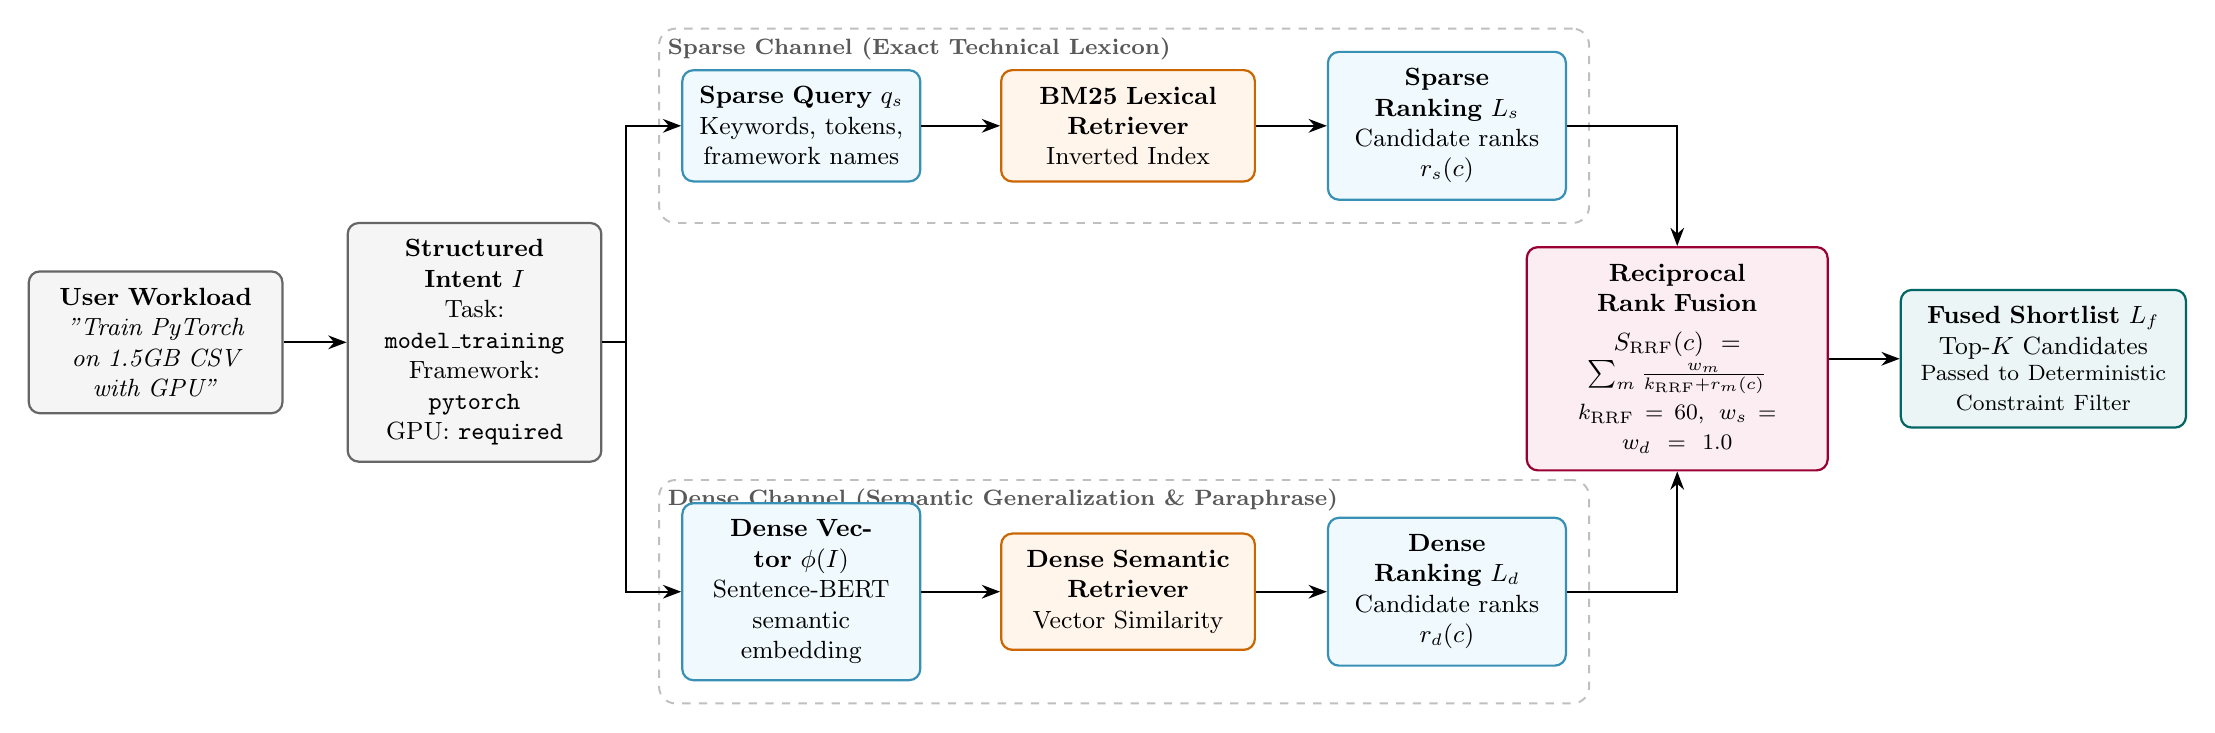
\begin{tikzpicture}[
    font=\small,
    >=Stealth,
    node distance=1.0cm and 0.8cm,
    box/.style={
        draw=blue!70!black,
        fill=blue!5,
        rounded corners=4pt,
        align=center,
        line width=0.8pt,
        inner sep=6pt,
        minimum height=0.9cm
    },
    querybox/.style={
        box,
        draw=gray!80!black,
        fill=gray!8,
        text width=2.8cm
    },
    indexbox/.style={
        box,
        draw=orange!80!black,
        fill=orange!8,
        text width=2.8cm
    },
    rankbox/.style={
        box,
        draw=cyan!70!black,
        fill=cyan!6,
        text width=2.6cm
    },
    fusionbox/.style={
        box,
        draw=purple!80!black,
        fill=purple!7,
        text width=3.4cm
    },
    outputbox/.style={
        box,
        draw=teal!80!black,
        fill=teal!8,
        text width=3.2cm
    },
    group/.style={
        draw=gray!50,
        dashed,
        rounded corners=6pt,
        line width=0.7pt,
        inner sep=8pt
    },
    grouplabel/.style={
        font=\footnotesize\bfseries,
        text=gray!70!black,
        anchor=north west
    }
]

% Inputs
\node[querybox] (query) {\textbf{User Workload}\\\textit{"Train PyTorch on 1.5GB CSV with GPU"}};
\node[querybox, right=of query] (intent) {\textbf{Structured Intent $I$}\\Task: \texttt{model\_training}\\Framework: \texttt{pytorch}\\GPU: \texttt{required}};

% Branching Queries
\node[rankbox, above right=0.5cm and 1.0cm of intent] (sparse_q) {\textbf{Sparse Query $q_s$}\\Keywords, tokens,\\framework names};
\node[rankbox, below right=0.5cm and 1.0cm of intent] (dense_q) {\textbf{Dense Vector $\phi(I)$}\\Sentence-BERT\\semantic embedding};

% Retrievers & Indexes
\node[indexbox, right=1.0cm of sparse_q] (sparse_idx) {\textbf{BM25 Lexical}\\\textbf{Retriever}\\\small Inverted Index};
\node[indexbox, right=1.0cm of dense_q] (dense_idx) {\textbf{Dense Semantic}\\\textbf{Retriever}\\\small Vector Similarity};

% Intermediate Rankings
\node[rankbox, right=0.9cm of sparse_idx] (sparse_rank) {\textbf{Sparse Ranking $L_s$}\\Candidate ranks\\$r_s(c)$};
\node[rankbox, right=0.9cm of dense_idx] (dense_rank) {\textbf{Dense Ranking $L_d$}\\Candidate ranks\\$r_d(c)$};

% RRF Fusion
\node[fusionbox, right=1.0cm of $(sparse_rank)!0.5!(dense_rank)$] (rrf) {
    \textbf{Reciprocal Rank Fusion}\\[3pt]
    $S_{\mathrm{RRF}}(c) = \sum_{m} \frac{w_m}{k_{\mathrm{RRF}} + r_m(c)}$\\[3pt]
    \footnotesize $k_{\mathrm{RRF}}=60,\; w_s=w_d=1.0$
};

% Fused Output
\node[outputbox, right=0.9cm of rrf] (shortlist) {
    \textbf{Fused Shortlist $L_f$}\\
    Top-$K$ Candidates\\
    \footnotesize Passed to Deterministic\\Constraint Filter
};

% Connectors
\draw[->, line width=0.8pt] (query) -- (intent);
\draw[->, line width=0.8pt] (intent.east) -- ++(0.3,0) |- (sparse_q.west);
\draw[->, line width=0.8pt] (intent.east) -- ++(0.3,0) |- (dense_q.west);

\draw[->, line width=0.8pt] (sparse_q) -- (sparse_idx);
\draw[->, line width=0.8pt] (dense_q) -- (dense_idx);

\draw[->, line width=0.8pt] (sparse_idx) -- (sparse_rank);
\draw[->, line width=0.8pt] (dense_idx) -- (dense_rank);

\draw[->, line width=0.8pt] (sparse_rank.east) -| (rrf.north);
\draw[->, line width=0.8pt] (dense_rank.east) -| (rrf.south);

\draw[->, line width=0.8pt] (rrf) -- (shortlist);

% Group Boxes
\begin{scope}[on background layer]
    \node[group, fit=(sparse_q) (sparse_idx) (sparse_rank), label={[grouplabel]north west:Sparse Channel (Exact Technical Lexicon)}] (g_sparse) {};
    \node[group, fit=(dense_q) (dense_idx) (dense_rank), label={[grouplabel]north west:Dense Channel (Semantic Generalization \& Paraphrase)}] (g_dense) {};
\end{scope}

\end{tikzpicture}
\end{document}
